\chapter{ОБЗОР ЛИТЕРАТУРЫ}\label{ch1}


\section{Общие сведения о плазме}

В любом газе некоторое количество атом ионизовано. Таким образом, в газе помимо нейтральных атомов с концентрацией $n_n$ содержатся и некоторое количество ионов и электронов, концентрации которых соответственно обозначают как $n_i$ и $n_e$. Ионы обычно только однократно ионизированы, т. е.
\begin{equation}
n_e \approx n_i^I.
\end{equation}
Вводится очень важный параметр --- степень ионизации газа. Он, очевидно, выражается как
\begin{equation}
k_c = \frac{n_e}{n_n}.
\end{equation}

При достаточно больших концентрациях и степени ионизации взаимодействие положительно и отрицательно заряженных частиц приводит к поддержанию макроскопической нейтральности в объемах, сравнимых по размеру с объемом газа; при этом нарушения макроскопической нейтральности приводят к появлению сильных электрических полей, быстро восстанавливающих ее. Ионизованный газ при таких концентрациях и называется \textit{плазмой}. Это название было предложено в 1923 г. И. Ленгмюром при изучении электрических разрядов в лампах заполненных ионизированным газом \cite{golant,kotelnikov2008}.


Плазма является самым распространенным известным на сегодняшний день состоянием вещества, в силу того, что все звезды, атмосферы планет и межзвездный газ по большей части находятся именно в состоянии плазмы. Помимо этого плазма --- это естественное состояние сильно разогретого вещества \cite{golant,archenovich}.

Температуру в физике плазмы принято изменять в энергетических единицах, а именно
\begin{equation}
\left[T\right] = \left[\text{эВ}\right].
\end{equation}
Везде далее под температурой будет иметься в виду именно энергетическая температура, если не указано иначе. Её связь с абсолютной температурой $T_K$ даётся выражением
\begin{equation}
T = k T_K,
\end{equation}
где $k$ --- постоянная Больцмана. Связь средней энергии теплового движения частиц $W$ с температурой плазмы, как и для любого равновесного газа с тремя степенями свободы, дается равенством
\begin{equation}
W = \frac{3}{2} T.
\end{equation}

Очень часто плазма является неравновесной. Для того, чтобы корректно описывать её поведение в подобных случая вводят две температуры: ионная температура $T_i$ и электронная температура $T_e$.

Как уже упоминалось выше, любое нарушение микроскопической нейтральности приводит к появления сильных полей, которые стремятся всё уравновесить. Однако, существует некоторый предельный объём, квазинейтральность внутри которого может быть свободно нарушена благодаря тепловому движению частиц плазмы. Простейшая оценка характерного расстояния при котором это происходит даёт следующее выражение:
\begin{equation}
r_D = \sqrt{\frac{T_e \varepsilon_0}{n_e e^2}},
\end{equation}
где $e$ --- элементарный заряд. Это величину называют \textit{радиусом Дебая}.

\section{Управляемый термоядерный синтез}

\subsection{Основные реакции}

Известна \cite{sivuhin5} экспериментальная зависимость удельной энергии связи $E_{\text{св}}/A$ ядра от количества нуклонов $A$ в этом ядре (рисунок \ref{fig:link_energy}).  Из анализа данной зависимости можно сделать вывод о существовании двух различных типов энергетически выгодных ядерных реакций: соединение (синтез) легких ядер и распад тяжелых ядер. Человечество хорошо освоило второй способ, доказательством тому служит существование множества АЭС. Однако, существует главная проблема --- недостаток сырья, тяжёлые элементы редки.

Синтез легких элементов имеет два основных преимущества: практически нескончаемые запасы топлива и более энергетически выгодная реакция. К минусам же относятся огромные технологические и инженерные проблемы при попытки его осуществления \cite{lukyanov}.

Проводить реакцию используя систему пушка-мишень не представлялось возможным, т. к. сечение реакции слишком мало. Лишь одна из многих тысяч ускоренных  частиц, падающих на мишень, вызывает ядерную реакцию. Остальные непроизводительно расходуют запасённую энергию малыми порциями на ионизацию и возбуждение атомов.

\begin{figure}[h]
\centering
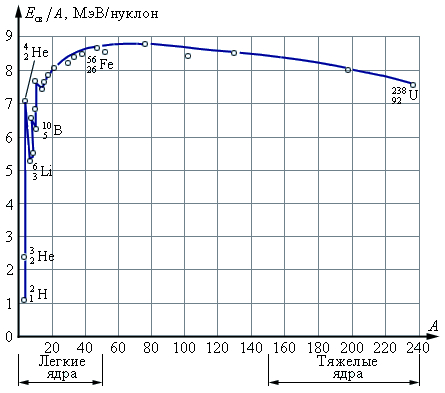
\includegraphics[width=0.7\linewidth]{../fig/ch1/link_energy}
\caption{Зависимость удельной энергии связи ядра от числа нуклонов в этом ядре}
\label{fig:link_energy}
\end{figure}

Тогда в 1950 г. И. Е. Таммом и А. Д. Сахоровым было предложено использовать следующую схему, в которой газ из необходимых элементов доводят до состояния плазмы со средней тепловой энергией движения достаточной для термоядерной реакции ( $W \sim 10 \div 100$ кэВ, энергия достаточная для преодоления кулоновского барьера). Далее, удержание полученной системы было предложено некой сложной \textit{магнитной ловушкой}.


Практический интерес представляют две известные реакции\cite{dnestrovsky}:
\begin{enumerate}
\item $D,D$-реакция. Может идти равновероятно одним из двух способов:
\begin{equation}
D + D \to
\begin{cases}
\left( ^3He + 0,82 \text{ МэВ}  \right) + \left( n + 2,45 \text{ МэВ} \right) \\
\left( T + 1,01 \text{ МэВ}  \right) + \left( p + 3,03 \text{ МэВ} \right)
\end{cases}.
\end{equation}
\item $D,T$-реакция:
\begin{equation}
D + T \to \left( ^4He + 3,52 \text{ МэВ}  \right) + \left( n + 14,06 \text{ МэВ} \right)
\label{eq:DT_rec}
\end{equation}.
\end{enumerate}

$D,T$-реакция сопровождается более интенсивным выделением энергии, а её сечение  в 50-100 раз превышает обе $D,D$-реакции, поэтому она более предпочтительна.

Стоит отметить, что значительную часть энергии получает нейтрон --- нейтральная частица. Отсутствие у неё заряда ставит большую проблему о том, как использоваться эту энергию, ведь электромагнитные поля здесь уже бессильны.

\subsection{Критерий Лоусона}

Необходимо прикладывать огромное количество энергии для того, чтобы удерживать горячую плазму достаточного объема и плотности. В 1957 году британским физиком Дж. Д. Лоусоном  был предложен оценочный критерий о положительном выходе термоядерной реакции \cite{Lawson}. Его рассуждения основывались на простом неравенстве
\begin{equation}
W_{\text{яд}} - W_{\text{тор}} - W_{\text{ост}} > 0, 
\end{equation}
где $W_{\text{яд}}$ --- энергия термоядерной реакции, $W_{\text{тор}}$ --- потери на тормозное излучение,  $W_{\text{ост}}$ --- остальные потери, которые некоторым пропорциональны $nT$. В своих рассуждениях Лоусон приходит к следующему неравенству:
\begin{equation}
n \tau > f(T) = \frac{T}{C_1 E_{\text{р}} <\sigma u> - C_2 \sqrt{T}},
\label{eq:Lowson_cr}
\end{equation}
где $E_{\text{р}}$ --- энергетический выход реакции, $u$ --- относительная скорость реагирующих ионов, $\sigma$ --- сечение реакции, $\tau$ --- характерное время удержания, $n$ --- концентрация ионов, $C_1,C_2$ --- некоторые константы. 

Функция $f(T)$ в правой части неравенства \eqref{eq:Lowson_cr} имеет минимум, так как при малых $T$ быстро уменьшается $<\sigma u>$, а при больших $T$ растёт числитель. Для $D,T$-реакции минимум функции находится \cite{kotelnikov} при $T_{\min} \approx 23 \text{ кэВ}$ (рисунок \ref{fig:f_T_Lowson}). 

\begin{figure}
\centering
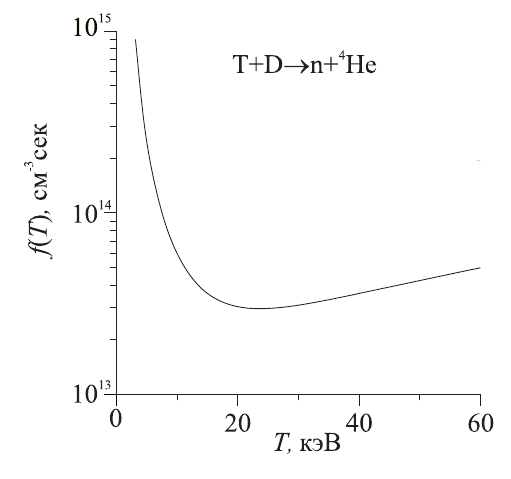
\includegraphics[width=0.5\linewidth]{./fig/ch1/f_T_Lowson}
\caption{График зависимости функции $f(T)$ для $D,T$-реакции}
\label{fig:f_T_Lowson}
\end{figure}


Одним из основных параметров любой ловушки является \textit{параметр удержания} $n \tau$.


\subsection{Некоторые характерные параметры плазменных ловушек}

В случае создания термоядерного синтеза, кроме критерия Лоусона \eqref{eq:Lowson_cr}, выделяют параметр $Q$, равный отношению выделяемой мощности реактора, к его потребляемой мощности. Таким образом, глобально ставится задача создания реактора с $Q>1$.

Также очень важным параметром является параметр $\beta$. Это есть отношение плазменного давления, к магнитному давлению в ловушке:
\begin{equation}
\beta = \frac{P_{plasma}}{P_{mag}} = \frac{nT}{B^2/2 \mu_0}.
\end{equation}

Для токамаков (установок с закрытой конфигурацией магнитного поля и торообразными магнитными поверхностями) выделяют ещё один параметр $q$ --- \textit{величина запаса устойчивости}. $q$ численно равняется отношению числа обходов $m$ по большому радиусу тора к числу $n$ обходов по малому радиусу тора. Если $q = m/n$ является простой дробью, то данный случай соответствует резонансной поверхности. А так как в сильном магнитном поле частицы дрейфуют вдоль магнитных силовых линий, то этот случай означает \textit{вырожденность магнитной линии}, от этого всегда стараются избавляться, т. к. это приводит к неустойчивости. 


\section{Обзор установок по удержанию горячей плазмы}

Анализируя критерий Лоусона \eqref{eq:Lowson_cr}, можно прийти к двум принципиально различным способам удержания плазмы. Во-первых, выражение в правой части для конкретной реакции имеет своё определенное минимальное значение, которое легче всего превзойти. Тогда очевидны два принципиально различных подхода для увеличения параметра удержания $n \tau$:
\begin{enumerate}
\item Большое время удержания, но небольшая плотность плазмы;
\item Малое время удержания, но высокая плотность плазмы. Данный способ носит название \textit{инерционного термоядерного синтеза}.
\end{enumerate}

В данной работе рассмотрен будет только первый способ. Установки по длительному удержанию плазмы классифицируют по их магнитной конфигурации, т. о. выделяют:
\begin{enumerate}
\item Открытые ловушки. Магнитные линии замкнуты вне ловушки;
\item Закрытые ловушки. Магнитные линии замкнуты внутри ловушки.
\end{enumerate}

Рассмотрим текущее состояние как открытых ловушек, так и закрытых. Стоит отметить, что множество проектов на данный момент уже закрыты, кризис пришёлся примерно на 1980-1990 гг. Рассмотрим только наиболее значимые из действующих проектов.

\subsection{Открытые ловушки}
\label{sec:open_trap}

\subsubsection{Амбиполярная ловушка GAMMA-10, Цукуба, Япония}

Самая крупная открытая ловушка находится в Цукубе, Япония --- это амбиполярная ловушка GAMMA-10. Её строительство было начато в 1980 г. \cite{gamma10_history} Проект активно развивается и в настоящее время.


\begin{figure}[h]
\centering
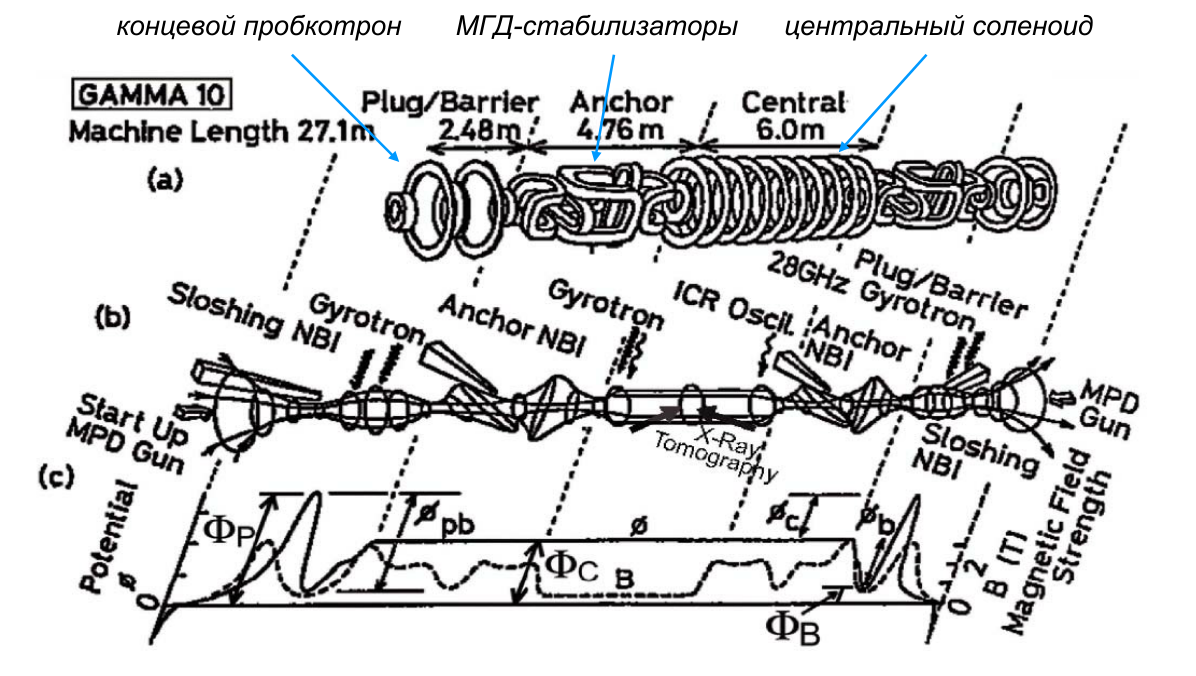
\includegraphics[width=0.9\linewidth]{./fig/ch1/GAMMA10}
\caption{Схематическое устройство амбиполярной ловушки GAMMA-10, Цукуба, Япония}
\label{fig:GAMMA10}
\end{figure}


GAMMA-10 состоит из центрального соленоида (основное место удержания плазмы), МГД-стабилизаторов и концевых пробкотронов для формирования запирающих потенциалов и термальной изоляции (рисунок \ref{fig:GAMMA10}). Нагрев и поддержание температуры плазмы производится двумя способами:
\begin{enumerate}
\item СВЧ нагрев (28 ГГц и 77 ГГц);
\item Инжекция горячих нейтралов.
\end{enumerate}
Радиационные потери сведены к минимуму благодаря аксиальной симметрии магнитного поля\cite{gamma10_review}.

Магнитное поле в центральном соленоиде 
\[
B_{\text{ц}} \approx 0,5 \text{ Тл},
\]
а на оси магнитных зеркал
\[
B_{\text{зер}} \approx 3,5 \text{ Тл},
\]
тогда пробочное соотношение установки будет составлять
\begin{equation}
R = \frac{B_{\text{зер}}}{B_{\text{ц}}} = 7.
\end{equation}
Такого высокого результата получается достигнуть благодаря т. н. катушкам <<бейсбольного>> типа.

Полная протяженность магнитной камеры составляет 27 метров, а её объём --- 180 м$^3$. Радиус центрального соленоида
\[
r = 0,36 \text{ м},
\]
а его протяженность 
\[
L = 6 \text{ м}.
\]
Основной СВЧ нагрев производится гиротроном на частоте 28 ГГц при мощности $1\div2$ МВт.
Последние эксперименты позволяют достичь плотности \cite{sumida2015high}
\[
n_e = 4,4 \cdot 10^{-18} \text{ м}^{-3}.
\] 
Максимальные температуры, которые получается достичь
\[
T_i = 4 \text{ кэВ}, \qquad T_e = 1 \text{ кэВ}.
\]

Последние исследования направлены на корреляцию ЭВМ вычислений, установку дополнительно регистрационного оборудования, разработка новых диверторных (поглощающих) мишеней\cite{imai2013gamma}.

Численные расчёты ведутся во многих направлениях \cite{gamma10_code}: расчёт магнитных полей, от систем сложной формы; расчёт траекторий единичных частиц; расчёт потока частиц при кулоновском взаимодействии и т.д. Методы расчёта также разнообразны --- это как и сеточные методы, методы частица-частицы, так и методы Монте-Карло.


\subsubsection{Установка ГОЛ-3, Новосибирск, Россия}

Установка <<ГОфрированная Ловушка>> (ГОЛ-3) --- открытая ловушка для удержания субтермоядерной плазмы. Основополагающая идея была предложена в 1971 г. Г. И. Будкером, В. В. Мирновым и Д. Д. Рютовым. Её особенностью является, как понятно из названия, \textit{гофрированная структура магнитного поля}. Такое поле формируется соединенными подряд пробкотронами.

\begin{figure}[h]
\centering
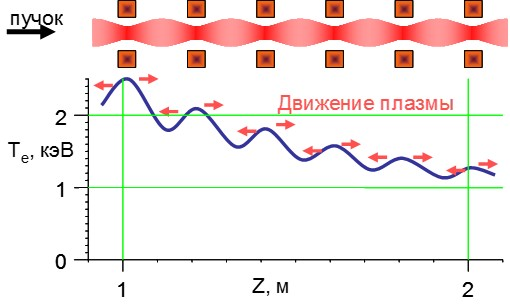
\includegraphics[width=0.7\linewidth]{./fig/ch1/GOL-3_02-03}
\caption{Неоднородный нагрев электронов и возникающие потоки плазмы на установке ГОЛ-3}
\label{fig:GOL-3_02-03}
\end{figure}


В такой системе заряженные частицы разбиваются на две группы: захваченные в одиночных пробкотронах и пролётные, попавшие в конус потерь одиночного пробкотрона (рисунок \ref{fig:GOL-3_02-03}). Если длина пробега частиц меньше размера ловушки, то при движении пролетных частиц через пробкотроны они начинают испытывать силу трения со стороны захваченных, что резко замедляет скорость разлета плазмы: вместо прямолинейного разлета движение частиц становится диффузионным \cite{gol3_review}.


Основной 12-метровый соленоид состоит из 55 пробкотронов длиной 22 см и пробочным отношением
\[
R = \frac{B_{\max}}{B_{\min}} = \frac{4,8 \text{ Тл}}{3,2 \text{ Тл}} = 1,5.
\]

Нагрев плазмы на установке осуществляется при помощи инжекции релятивистских электронных пучков в предварительно созданную дейтериевую плазму. Электроны   вытягиваются из взрывоэмиссионного катода и ускоряются в ленточном диоде до энергии порядка 1 МэВ. Созданный мощный ($I \approx 50$ кА) релятивистский пучок сжимается и инжектируется в основной соленоид, где в дейтериевой плазме с плотностью 
\[
n = 10^{20} \div 10^{22} \text{ м}^{-3}
\]
вследствие развития двухпотоковой неустойчивости возникает большой уровень микротурбулентности и пучок теряет до $40\%$ своей энергии, передавая её электронам плазмы. Особенностью пучково-плазменного взаимодействия является высокий уровень турбулентности, что приводит к сильному (более $10^3$ раз) подавлению электронной теплопроводности. Это не даёт электронам плазмы остыть на торцах установки. Темп нагрева очень высокий --- за $3 - 4$ мкс плазменные электроны нагреваются вплоть до температуры 
\[
T_e \approx 5 \text{ кэВ},
\]
что является мировым рекордом для открытых ловушек. После окончания инжекции пучка (12 мкс) теплопроводность становится классической и электроны быстро остывают. Максимально достигнутая ионная температура \cite{gol3_prog}
\[
T_i \approx 3 \text{ кэВ}.
\]


Главной отличительной особенностью по сравнению с токамаками --- это более высокая плотность плазмы, однако, меньшая температура и время удержания. На данный момент усилия научной группы установки ГОЛ-3 направленны на внедрение системы нагрева горячими нейтралами.


\subsubsection{Установка ГДЛ, Новосибирск, Россия}


Установка ГДЛ (газодинамическая ловушка) создана в Новосибирском институте ядерной физики в 1986 году.  Эксперименты проводятся по настоящее время.


\begin{figure}[h]
\centering
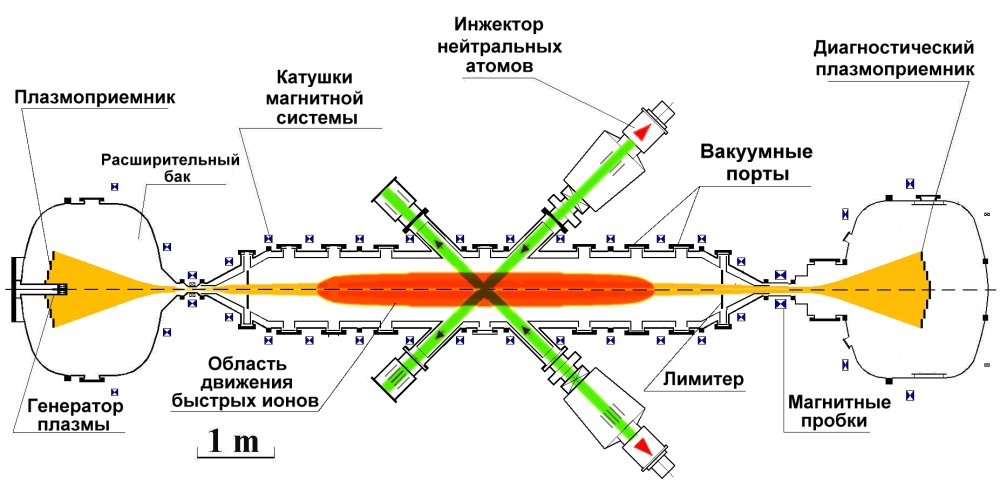
\includegraphics[width=0.95\linewidth]{../fig/ch1/GDL1}
\caption{Схема установки ГДЛ}
\label{fig:GDL1}
\end{figure}

Схема установки ГДЛ приведена на рисунке \ref{fig:GDL1}. Главной ее частью является осесимметричный пробкотрон длиной
\[
L = 7 \text{ м},
\] 
с полем $B_{\min} = 0,3$~Тл в центре и до $B_{\max} = 13$~Тл в пробках (т.е. пробочное соотношение $R = B_{\max}/B_{\min} \approx 43$), предназначенный для удержания двухкомпонентной плазмы. Одна компонента --- тёплая ($W \approx 200 \text{ эВ}$ и $n \approx 5 \cdot 10^{19} \text{ м}^{-3}$) плазма-мишень, а вторая быстрые ионы с $W \approx 10 \text{ кэВ}$ и $n \approx 5 \cdot 10^{19} \text{ м}^{-3}$. 

Стоит отметить, что в открытых ловушках большое увеличение пробочного отношения не даёт сильного прироста ко времени удержания, потому что \cite{dimov2005} зависимость логарифмическая
\[
\tau \sim \ln R.
\]

Важнейшим достоинством ГДЛ является простая и надежная физика продольного удержания плазмы, продольные потери частиц в ГДЛ практически не зависят от скорости их рассеяния внутри ловушки \cite{gdl_review}. Однако, чтобы получить нужное для реакторных приложений время удержания, достаточно увеличить пробочное отношение, насколько это позволительно, и увеличить длину ловушки до нужных размеров. Другим достоинством газодинамической ловушки является возможность достижения МГД устойчивости плазмы в рамках осесимметричной конфигурации магнитного поля при реализации механизма так называемого <<вихревого транспортного барьера>> \cite{beklemishev2010vortex}.

Нагрев плазмы осуществляется тремя основным способами: метод СВЧ нагрева или метод электронно циклотронного резонанса (ЭРЦ), инжекции высокого энергетический электронов и инжекции горячих нейтралов.

Важно отметить, что газодинамическая ловушка обладает еще одним очень важным достоинством, характерным для пробкотронов. Согласно результатам теоретического анализа МГД устойчивость в ГДЛ сохраняется при высоких значениях $\beta = 0,3 \div 0,7$.

В рамках экспериментальной программы ГДЛ ведется постоянная работа по повышению устойчивости плазмы, уменьшению и подавлению продольных потерь плазмы и энергии из ловушки, исследованию поведения плазмы в различных условиях работы установки, повышению температуры мишенной плазмы и плотности быстрых частиц.


Что касается численных кодов, то используются два основных крупных кода:
\begin{enumerate}
\item \textbf{ITCS}. Монте-Карло транспортный код для моделирования динамики быстрых ионов МСFIT (Monte-Carlo Fast Ion Transport Code) включает в себя различные модули, которые используют теорию парных кулоновских столкновений и уравнения классической магнитной гидродинамики.  

\item \textbf{DOL}. Код DOL (Длинные Открытые Ловушки) предназначен для описания нестационарных плазменных процессов в осесимметричных открытых ловушках. Решается кинетические уравнения.Присутствует усреднение баунс--колебаний. Присутствует также возможность расчёта интеграла столкновений для вычисления вида функции распределения быстрых ионов с использованием немаксвелловской рассеивающей функции и возможность расчёта продольных потоков частиц и энергии фоновой плазмы в режимах удержания с длиной свободного пробега частиц порядка длины установки \cite{DOL_code}.
\end{enumerate}


\subsection{Закрытые ловушки}

С самого начала развития науки об УТС (примерно 1950-е годы) было предложено две принципиально различные установки закрытого типа \cite{Kubic2007}:

\begin{enumerate}
\item Стелларатор. Стелларатор был изобретен Л. Спитцером в 1951 г. в Принстонском университете, США. Магнитное поле в установке \textit{полностью создаётся внешними катушками}, что, помимо прочего, позволяет использовать его в непрерывном режиме. Его силовые линии подвергаются вращательному преобразованию, в результате которого эти линии многократно обходят вдоль тора и образуют систему замкнутых вложенных друг в друга тороидальных магнитных поверхностей (рисунок \ref{fig:W7X-Spulen_Plasma_blau_gelb}). Таким образом, с помощью сложной конфигурации поля снимается вырождение магнитных линий.

\begin{figure}[h!]
\centering
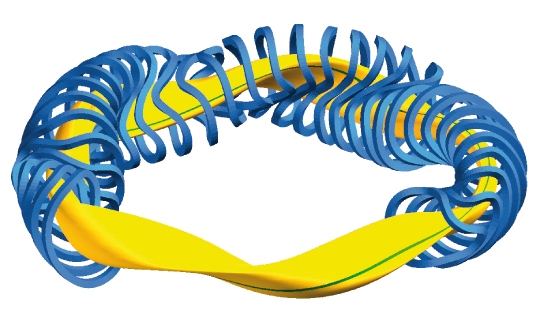
\includegraphics[width=0.5\linewidth]{./fig/ch1/W7X-Spulen_Plasma_blau_gelb}
\caption{Схематическое изображения плазменного шнура и магнитных катушек стелларатора}
\label{fig:W7X-Spulen_Plasma_blau_gelb}
\end{figure}


\item Токамак. Принципиальная схема токамака была предложена Таммом и Сахаровым в 1952 г в России. Магнитное поле в установке создаётся тремя способами: катушками тороидального поля, катушками полоидального поля и непосредственно самим плазменным током (рисунок \ref{fig:tokamak}). Большую роль в снятии вырождения магнитных линий играет именно наличие плазменного тока --- это и есть основное отличие токамака от стелларатора. 
В современном токамаке форма плазменного шнура обычно является D-образной, потому что именно при такой конфигурации повышается устойчивость плазмы.

\begin{figure}[h!]
\centering
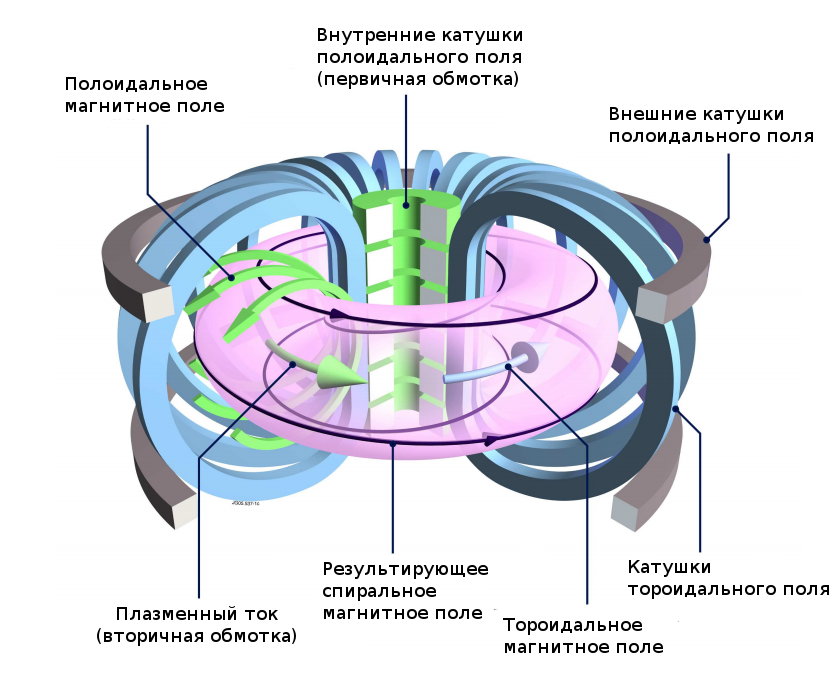
\includegraphics[width=0.75\linewidth]{./fig/ch1/tokamak}
\caption{Устройство токамака}
\label{fig:tokamak}
\end{figure}

\end{enumerate}


Закрытые системы имеют гораздо большую популярность среди существующих и существовавших проектов \cite{plasma_nsu} (рисунок \ref{fig:plasma_in_different_places}). 


\begin{figure}[h]
\centering
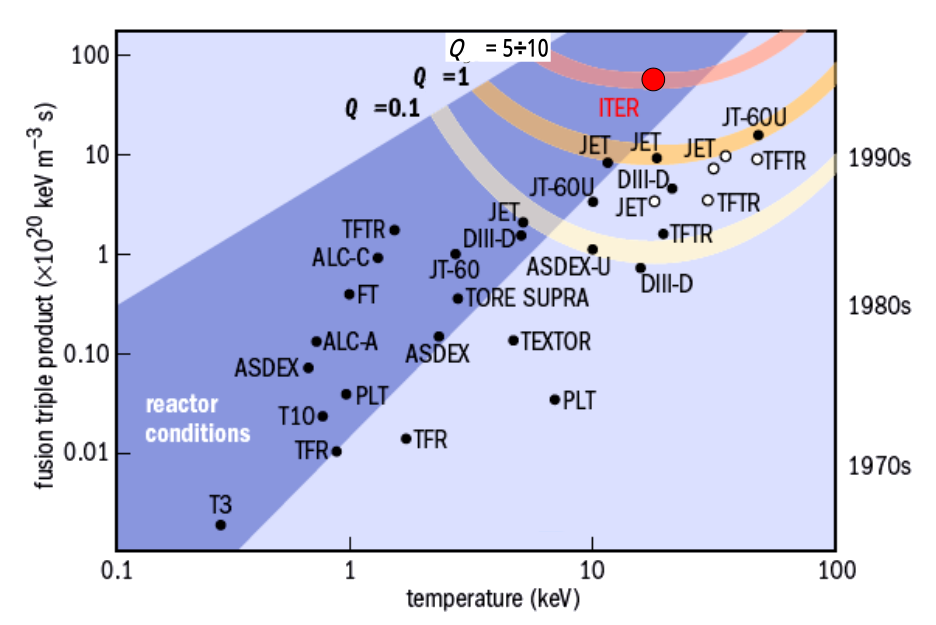
\includegraphics[width=0.8\linewidth]{./fig/ch1/plasma_in_different_places}
\caption{Критерий Лоусона для различных установок по УТС}
\label{fig:plasma_in_different_places}
\end{figure}


Приведём основные действующие установки на настоящий момент:
\begin{enumerate}
\item \textit{Токамак Joint European Torus (JET), Оксфордшир, Англия.} Самый крупный в мире действующий токамак, созданный организацией Евратом в Великобритании. В нём использован комбинированный нагрев: 20 МВт --- нейтральная инжекция, 32 МВт --- ионно-циклотронный резонанс. В итоге, критерий Лоусона лишь в 4—5 раз ниже уровня зажигания \cite{Kubic2007}.
\item \textit{Стелларатор Wendelstein 7-X, Грайфсвальд, Германия.} Проект завершился в 2014 году. Целью создания являлась проверка практической пригодности термоядерного реактора типа стелларатор. Первая тестовая плазма была получена в декабре 2015 года \cite{Max_plankINST}.
\item \text{Токамак JT-60SA, Япония.} Логическое продолжение установок JT-60 и JT-60U. Проект является частью крупного проекта ITER. Создан для оптимизации основного проекта \cite{JT-60SA}.
\item \textit{Experimental Advanced Superconducting Tokamak (EAST), Китай.} Экспериментальный усовершенствованный сверхпроводимый токамак. Работает в рамках международного проекта ITER. Была впервые получена реакция с параметром $Q = 1,25$ в 2007 году \cite{wan2009recent}.
\item \textit{Сферомак Глобус-М, Санкт-Петербург, Россия.} Первый и единственный в России и один из первых в мире сферических токамаков (отношение большого и малого радиуса тора $R/a = 1,5$). Был введен в эксплуатацию в 1999 году \cite{globus-m}.
\item \textit{Токамак Т-15, Москва, Россия.} Является одной из крупнейших в мире экспериментальных термоядерных установок. Уникальность установке придает наличие крупнейшего в мире сверхпроводникового ниобий-оловянного тороидального магнита \cite{T15}.
\item И др.
\end{enumerate}

%\cite{Ryzhkov2015d}

\section{Моделирование плазмы. Обзор численных методов}

Теоретическое описание плазмы далеко не тривиально и ставит большое количество сложных и нелинейных задач, для решения которых приходится использовать компьютерное моделирование. В большинстве задач число частиц огромно и, разумеется, не представляется возможным на данный момент развития ЭВМ описать их все без каких либо упрощений. Так как в крупных исследованиях ставятся задачи с самосогласованными электромагнитными полями, сложными граничными условиями и т. д., методы использующие подходы из первых принципов (например, PP метод, он же метод молекулярной динамики) не имеют большой популярности среди настоящих работ. Действительно, нельзя просто создать внешнее стационарное поле, его придётся пересчитывать на каждом шаге, кроме того, вообще говоря, каждая частица взаимодействует с каждой, а при высоких энергиях в роль вступают времена запаздывания и релятивизм \cite{Flower2007}.

Однако, различные численные подходы позволяют значительно снизить объём вычислений. Каждый метод изначально создавался, чтобы корректно описывать систему в определённых пространственно-временных пределах \cite{Miloch2014}: в очень малых масштабах на первый план выходят методы частиц (PIC, PP) и кинетические подходы; в то время как в крупных масштабах выгоднее использовать методы магнитогидродинамики (MHD). Нередко задачу разбивают области и применяют гибридные методы.


\subsection{PP метод}

При моделировании плазмы методом частица-частица (метод молекулярной динамики) рассчитывается движение всех частиц с учётом взаимодействия каждой частицы со всеми (или почти со всеми) остальными. Рассмотрим этот метод в очень общих чертах, более подробное описание дано в главах \ref{ch2} и \ref{ch3}. Уравнение движения $i$-й частицы имеет вид:
\begin{equation}
\frac{d \vec{p_i}}{dt} = \vec{F}_{ex} (\vec{r}_i) - \sum\limits_{j \neq i} \nabla U_{ij} (r_{ij}),
\end{equation}
где $\vec{p}_i$ --- импульс $i$-й частицы, $\vec{F}_{ex}$ --- внешняя сила, $U_{ij}$ --- потенциал взаимодействия $i$-й частицы с $j$-й. Вид потенциала может сильно изменятся в силу поставленной задачи. В плазме поле одной частицы экранировано коллективным полем других. Экранированный потенциал можно представить в виде
\begin{equation}
U^*_{ij} = U_{ij} \Phi \left(  \frac{r_{ij}}{a} \right),
\end{equation}
где $a$ --- характерная длина экранировки. Для дебаевской экранировки в плазме~\cite{Flower2007}
\begin{equation}
\Phi \left(  \frac{r_{ij}}{a} \right) = e^{- r_{ij}/r_D}.
\label{eq:debai1}
\end{equation}

Интегрирование уравнения движения необходимо производить с достаточно малым шагом, много меньшем времени столкновений.

Для уходя от большого количества частиц использую метод укрупнения, то есть выполняют переход
\begin{equation}
\begin{cases}
m_i \\
q_i
\end{cases} \Longrightarrow 
\begin{cases}
M_i = N m_i \\
Q_i = N q_i
\end{cases},
\label{eq:Huge_par}
\end{equation}
где $N$ --- коэффициент укрупнения.

Данный метод часто используют для описания потоков заряженный частиц в вакууме, где необходимо рассмотреть тонкие релятивистские эффекты \cite{Kravchenya2010,Kovtun2010,Kovtun2005}.

\subsection{PIC метод}

Метод Particle-in-Cell (частица в ячейке) на данный момент имеет наибольшую популярность в изучении динамики плазмы. Метод относится к методам частиц --- плазма представляется в виде совокупности крупных частиц \eqref{eq:Huge_par}, для которых решается уравнение движения. Однако для нахождения самосогласованного электромагнитного поля изучаемый объём разбивается на пространственно-временную решётку, в котором разрешается система уравнений Максвелла:
\begin{eqnarray}
\Rot \vec{B} = \mu_0 \vec{j} + \frac{1}{c^2} \dfrac{\partial \vec{E}}{\partial t}, &\qquad& \Rot \vec{E} = - \dfrac{\partial \vec{B}}{\partial t}, \label{eq:Maxwell1} \\ \nonumber \\
\Div \vec{B} = 0, &\qquad& \Div \vec{E} = \dfrac{\rho}{\varepsilon_0}, \label{eq:Maxwell2}
\end{eqnarray}
где $\vec{j}$ --- плотность электрического тока, $\rho$ --- плотность электрического заряда. К уравнениям Максвелла также добавляется уравнение непрерывности
\begin{equation}
\Div \vec{j} + \parder{\rho}{t} = 0.
\label{eq:conti}
\end{equation}

Для численного решения первой пары уравнений Максвелла \eqref{eq:Maxwell1} зарекомендовал себя метод конечных разностей во временной области FDTD (finite-difference time-domain). 
Метод FDTD был разработан Кейном Йи в 1966 году \cite{yee1966numerical}. В основу метода был положена явная конечно-разностная схема второго порядка. Базовый алгоритм Йи для решения уравнений Максвелла предполагал дискретизацию электрической и магнитной компонент поля со сдвигом сеток друг относительно друга на полшага, как в пространственных координатах, так и по времени. Такой подход позволяет увеличить точность расчетов без увеличения числа звеньев сетки. Впоследствии алгоритм был модифицирован различными авторами, последние из работ это \cite{melo2009computational,chaudhury2010computational,de2002solving,Rylander200075}.

Основной алгоритм заключается в следующем \cite{dawson1983particle}. Существует пространственная решётка, на решётках её ячеек решается уравнение максвелла методом FDTD.  Зная поля $\vec{E}$ и $\vec{B}$, можно вычислить положение частицы в следующий момент времени. Зная положения и скорости частиц, можно вычислить $\rho$ и $\vec{j}$, а уже зная их можно опять считать поля. Основная проблема и различия между алгоритмами заключается именно в решении уравнения непрерывности \eqref{eq:conti}. На этом шаге в литературе встречаются очень много неявных выкладок об аппроксимации функции плотности $\rho$, которые явно не несут под собой  физического обоснования.


\begin{figure}
\centering
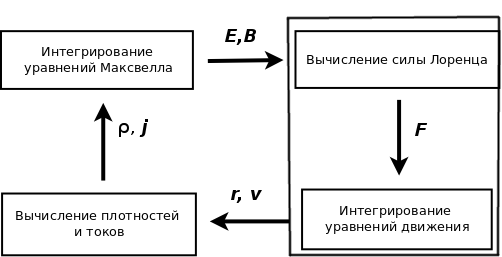
\includegraphics[width=0.8\linewidth]{./fig/ch1/PIC_al}
\caption{Упрощенный алгоритм метода PIC}
\label{fig:PIC_al}
\end{figure}



Современные алгоритмы позволяют добиться сложности вычислений $\mathscr{O} \left( n \ln n_g \right)$, где $n$ --- число частиц, $n_g$ число узлов решётки. Одним из быстрейших алгоритмов является алгоритм Такаяши Умеда \cite{umeda2003new}. В нём предложена т.н. схема аппроксимации зигзаг.

Устойчивость PIC метода, как и любого другого сеточного метода, определяется критерием Куранта
\begin{equation}
1 \geqslant \left(c dt \right)^2 \left( \frac{1}{dx^2} + \frac{1}{dy^2} + \frac{1}{dz^2} \right),
\label{eq:Kurant}
\end{equation}
где $dt$ --- шаг дискретизации по времени, а $dx,dy,dz$ --- шаг пространственной дискретизации.


\subsection{Кинетический подход}

В основе данного метода лежит уже не Лагранжев подход, а Эйлеров. 

Кинетическое уравнение выводится при рассмотрении функции распределения $f \left( \vec{r} (t), \vec{v} (t); t \right)$ в фазовом пространстве $\left\{ x,y,z,v_x,v_y,v_z \right\}$. Согласно теореме Лиувилля фазовый объём при движении в макроскопическом потенциальном поле остаётся постоянным:
\begin{equation}
\frac{d f}{dt} = 0.
\label{eq:kin1}
\end{equation}
При учёте взаимодействия частиц друг с другом в правой части \eqref{eq:kin1} запишется некоторый функционал $\Omega (f)$, который носит название интеграла столкновений \cite{chang1992unified}. Если раскрыть дифференциал в левой части \eqref{eq:kin1}, то в силу того, что $\vec{v} = \vec{v}(t)$, появится слагаемое вида $\partial \vec{v} / \partial t$, что является силой с точностью до константы в дорелятивистском случае. Подставив силу Лоренца, можно получить следующее выражение:
\begin{eqnarray}
\parder{f}{t} + \vec{v} \cdot \parder{f}{\vec{r}} + \frac{q}{m} \left( \vec{E} + \vecmult{v}{B} \right) \parder{f}{\vec{v}} = \Omega (f).
\label{eq:kinetic2}
\end{eqnarray}
Уравнение обычно дополняют системой Максвелла \eqref{eq:Maxwell1}, \eqref{eq:Maxwell1}. Такая система носит название \textit{уравнений Максвелла-Власова}.

Конкретный вид интеграла столкновений может быть различным, но самым распространённым его представлением является BGK приближение или $\tau$-приближение:
\begin{equation}
\Omega = \frac{f^{eq} - f}{\tau},
\label{eq:BGK}
\end{equation}
где $f^{eq}$ --- равновесная функция распределения, обычно используют Максвелловское распределение; $\tau$ --- характерное время релаксации.

В качестве методов решения, в последнее время очень активно развивается т. н. метод решёточных уравнений Больцмана (LBM). Последние достижения были сделаны М. Мендозой и Дж. Д. Мюнозом. Они предложили модифицировать существующий метод решения кинетических уравнения для жидкости и решать с помощью него систему уравнений Власова \cite{Mendoza2010,Romatschke2011,Mendoza2011,Mendoza2008,Hupp2011}. Стоит заметить, что в работе \cite{Mendoza2010} был проведено сравнение алгоритма Йи и алгоритма Мендозы. Результаты показали, что методы LBM менее ресурсозатратны и более быстрые.

Всё чаще встречаются работы, использующие кинетические подходы для описания горячей плазмы \cite{Pattison2008}. Например, работа \cite{Zhang2007} посвящена описанию горячей плазменной струи.

\begin{figure}
\centering
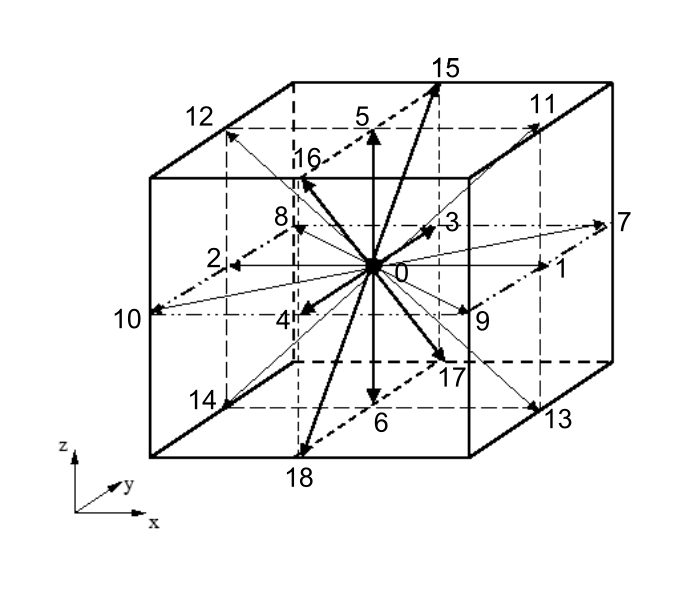
\includegraphics[width=0.6\linewidth]{./fig/ch1/D3Q19}
\caption{Трёхмерная решётка с 19-ю возможными направлениями D3Q19 в методе LBM}
\label{fig:D3Q19}
\end{figure}

В основе численного решения уравнения \eqref{eq:kinetic2} лежит раздробление моделируемого пространства на сетку. Далее, производится дискретизация основного уравнения --- в каждой ячейке частицы имеют ограниченное количество возможных направлений (рисунок \ref{fig:D3Q19}). Например, для моделирования в трёх изменениях наиболее распространена решётка типа D3Q19.

Численное решение происходит в два этапа:
\begin{enumerate}
\item Этап распространения. Продвижение всех потоков во всех возможных направлениях.
\item Столкновительный этап. Пересчитав макроскопические параметры каждой из ячеек, такие как скорость и плотность, высчитывается равновесная функция для полученных параметров $f^{eq}$, т.е. к чему должна стремится $f$ согласно \eqref{eq:BGK}.
\end{enumerate}

Более подробные математические выкладки выходят далеко за рамки данной работы. Здесь рассмотрены только лишь основные принципы и положения.

\subsection{MHD метод}

Когда пространственные и временные масштабы велики, то есть возможность значительно упростить уравнения Максвелла и представить плазму в виде некой сверхпроводящей жидкости. Такой подход носит название магнитогидродинамики (MHD).

Сверхпроводимость означает, что как только где-то появляется неоднородность зарядовой плотности, то она сразу исчезает благодаря почти идеально проводимости. Если характерная скорость в системе много меньше скорости $c$, то тогда можно пренебречь током смещения, а чтобы система оставалось полной её дополняют дифференциальным законом Ома:
\begin{equation}
\vec{j} = \sigma \left( \vec{E} + \vecmult{v}{B}  \right).
\end{equation}
Часто используют предел идеально проводящей плазмы при $\sigma \to + \infty$, $\vec{E} = - \vecmult{v}{B}$. Второе условие необходимо для того, чтобы $\vec{j}$ была конечно величиной.

Полная система уравнения магнитогидродинамики выглядит следующим образом:
\begin{eqnarray}
\parder{\rho}{t} + \Div \rho \vec{v} &=& 0, \\
\rho \left[  \parder{\vec{v}}{t} + \left( \vec{v} \cdot \nabla \right) \vec{v}  \right] &=& - \nabla p + \vecmult{j}{B}, \\
\Rot \vec{B} &=& \mu_0 \vec{j}, \\
\Rot \vec{E} &=& - \parder{\vec{B}}{t}, \\
p &=& F(\rho) , \\
\vec{j} &=& \sigma \left( \vec{E} + \vecmult{v}{B}  \right), \\
\Div \vec{B} &=& 0,
\end{eqnarray}
где $\rho$ --- плотность плазмы.

Численное решение производится методами как с помощью PIC кодов, так и LBM \cite{Pattison2008}  и другими методами \cite{Galanin2014}.

\subsection{Гибридные методы}

Существует возможность создания и гибридных методов, которые считают в себе  перечисленные выше подходы. Такие методы часто используются для исследования продолжительных явлений и значительно ускоряют процесс моделирования благодаря принятым упрощениям. Например, основываясь на том, что $v_e \gg v_i$, можно прийти к выводу, что для электронов использовать PIC код, а для расчёта эволюции ионов --- кинетический подход \cite{Miloch2014}. Однако, в таких случаях надо быть всегда предельно внимательным при <<сшивке>> методов.

